\documentclass{article}
\usepackage{graphicx}
\usepackage{listings}
\usepackage{color}
\graphicspath{ {images/} }

\definecolor{mygreen}{rgb}{0,0.6,0}

\lstset{ %
	basicstyle=\footnotesize,        % the size of the fonts that are used for the code
	breakatwhitespace=false,         % sets if automatic breaks should only happen at whitespace
	breaklines=true,                 % sets automatic line breaking
	captionpos=b,                    % sets the caption-position to bottom
	commentstyle=\color{mygreen},    % comment style
	deletekeywords={...},            % if you want to delete keywords from the given language
	escapeinside={\%*}{*)},          % if you want to add LaTeX within your code
	extendedchars=true,              % lets you use non-ASCII characters; for 8-bits encodings only, does not work with UTF-8
	frame=single,	                 % adds a frame around the code
	keepspaces=true,                 % keeps spaces in text, useful for keeping indentation of code (possibly needs columns=flexible)
	keywordstyle=\color{blue},       % keyword style
	language=Java,                 	 % the language of the code
	otherkeywords={*,...},           % if you want to add more keywords to the set
	numbers=left,                    % where to put the line-numbers; possible values are (none, left, right)
	numbersep=5pt,                   % how far the line-numbers are from the code
	showspaces=false,                % show spaces everywhere adding particular underscores; it overrides 'showstringspaces'
	showstringspaces=false,          % underline spaces within strings only
	showtabs=false,                  % show tabs within strings adding particular underscores
	stepnumber=5,                    % the step between two line-numbers. If it's 1, each line will be numbered
	tabsize=2,	                     % sets default tabsize to 2 spaces
}



\begin{document}
	\title{Hybrid Images}
	\author{Bradley Mason}
	\maketitle
	
	\section*{Convolution Algorithm}
	In my algorithm{\tiny Pg.3} I take the image and produce an empty array the size of the original image. I then use two for loops to loop through each pixel in the original image, set a sum variable to 0 and then loop through the points in the kernel. For each point in the kernel add a value to the sum variable. The variable is determined by a two step process, the first being to find the corresponding pixel of the original image within the kernel and the second is to multiply it by the correct weighting.
	\\
	To visualise this you can image that the current image pixel is the centre point of the kernel and to find the point in the kernel that the loop is currently on, we add a modifier to the pixel location. That modifier is the current co-ordinate in the kernel’s scope, minus the floor of half of the kernels width and minus another 1 because the indexing starts at 0. For example, if we have a kernel of size 5x5 and we wish to find the pixel in the top left corner of the kernel (0,0) we add to the image pixel’s x co-ordinate 0-2(floor of half kernels width 5). This gives us the pixel two to the left and we then do the same to the y co-ordinate to give us 2 upwards.\\
	We would then find the weighting stored at that point in the kernel and multiply the value of the pixel in the original image at the location we just found. We then add this value to the sum, once we have summed up all the pixel values with their weighting modifiers we store the resultant value in the empty array in the current x,y co-ordinates of the for loop. At the end I convert the array into an FImage object and normalise it. I used the array because I timed the code and found them to be 10\% faster than using an FImage throughout.\\
	There is an extra feature here, I have allowed the kernel to attempt to find pixels outside of the range of the image which I catch with a try catch clause and ignore. This means that for pixels less than half a kernel width from the edge, the convolution will not be able to use the full sum of all the kernel points but rather a partial sum, this creates a blending effect that without this (as I initially tried) you have a sharp border of un-altered pixels. I personally felt the blended effect gives a more pleasing result and also provides a closer match to the sample provided in the coursework specification.
	
	\section*{Hybrid Images Algorithm}
	To begin with I collect the two images and create a copy of the image I intend to use for the high pass. I then specifiy a constant sigma for the kernel and calculate the size accordingly. I utilise the OpenIMAJ library to produce a kernel with these variables. I instantiate my convolution class, then convolute the first image I collected to produce my low pass image. I then convolute the copy of the second image and subtract the result from the original second image, this gives me my high pass image. I then add the pixel values of the high and low pass images using OpenIMAJ’s library to give my final resultant hybrid image. I then loop through the pixels and set any border pixels to black, I try to speed this up by using an if statement where if the image is square it reduces the time complexity of the loops from $N^2$ to N by removing the need of the imbedded for loop. I attempted this in multiple ways using the OpenIMAJ library rather than a for loop (for example by drawing the image without it’s edge pixels onto a black background) however none of the methods were faster than the for loops worst case time.
	With all the image manipulation completed the code moves on to displaying the results, I build a frame big enough to fit all the images on and set it to be white. I then progress through and draw on each stage of image processing from the original all the way to the final result; I label each of these images too. Finally, to demonstrate that the image does what it is intended I display several copies of the original image halving in size each time to give the same effect as moving further away.\\
	Throughout this class I print updates to the terminal with times for reference of progress.
	
	\section*{Results}
	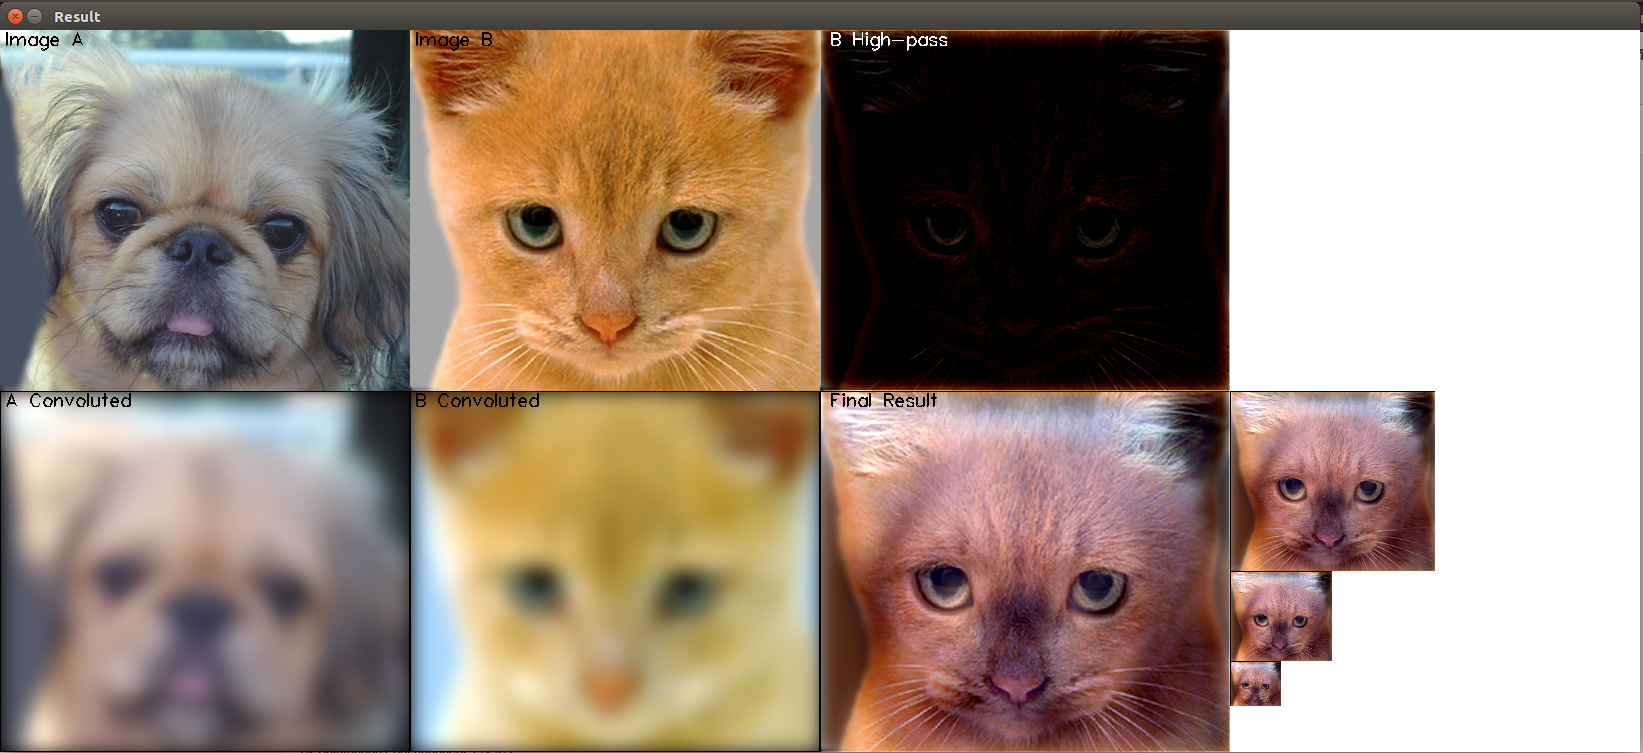
\includegraphics[scale=0.21]{hybrid_image}
	From the samples provided you can see that this does indeed work; these image are produced with a sigma value of 10 which I obtained by trying different values and this seemed to achieve the best results without being too slow. On another page below I have included another sample output I found worked rather well.
	
	\section*{Convolution Code}
	\begin{lstlisting}
	public void processImage(FImage image) {
		
		// convolve image with kernel and store result back in image
		
		//Define some variables about the image for later calculations
		irows = image.getRows();
		icols = image.getCols();
		trows = kernel.length;
		tcols = kernel[0].length;
		
		//Produce a temporary black image to store the convoluted pixels
		float temp[][] = new float[image.height][image.width];
		
		trhalf = (int) Math.floor(trows/2);
		tchalf = (int) Math.floor(tcols/2);
		
		//Loop through all pixels of the original image
		for (int x = 1; x<icols-1; x++) {
			for (int y = 1; y<irows-1; y++) {
				//Reset the sum
				float sum = 0;
				//Loop through all points within the kernel
				for (int iwin = 1; iwin<trows; iwin++) {
					for (int jwin = 1; jwin<tcols; jwin++) {
						try {
							//Add to the sum the value of the current image pixel multiplied by the weighting in that location of the kernel
							modx = x+iwin-trhalf-1;
							mody = y+jwin-tchalf-1;
							sum += image.pixels[mody][modx]*kernel[jwin][iwin]; 
						} catch(Exception e) {}
					}
				}
			//Set the corresponding blacked out image's pixel to the final summed value
			temp[y][x] = sum;
			}
		}
		//Normalise and return the convoluted image
		FImage ret = new FImage(temp);
		image.internalAssign(ret.normalise());
	}
	\end{lstlisting}
	\section*{Second Hybrid Image Sample}
	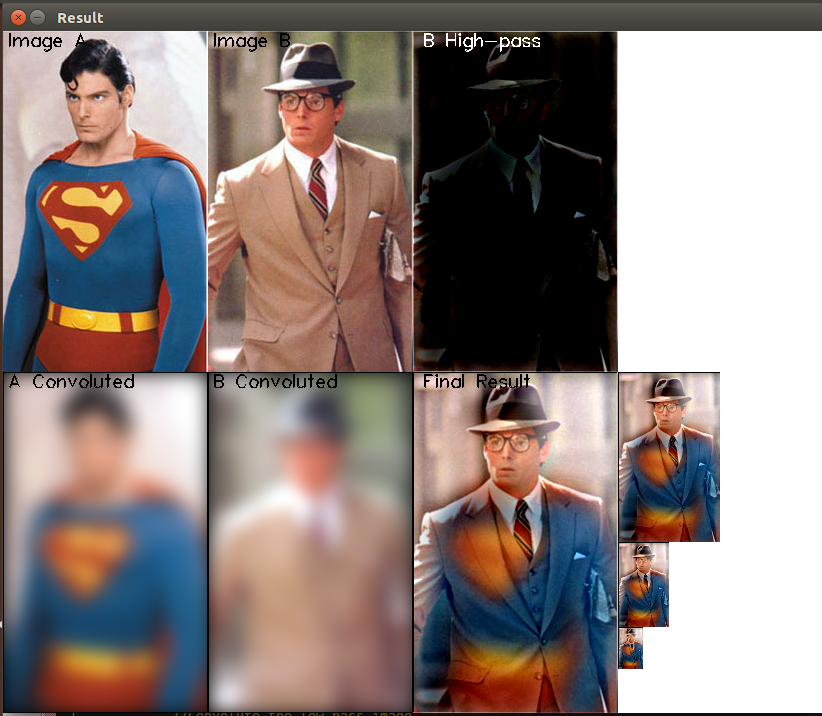
\includegraphics[scale=0.45]{second_hybrid}
	\footnote{"http://www.superhero-therapy.com/wp-content/uploads/2015/02/Superman-ClarkKent-ChrisReeve.jpg"}
\end{document}